\documentclass[11pt]{aghdpl}
% \documentclass[en,11pt]{aghdpl}  % praca w języku angielskim

% Lista wszystkich języków stanowiących języki pozycji bibliograficznych użytych w pracy.
% (Zgodnie z zasadami tworzenia bibliografii każda pozycja powinna zostać utworzona zgodnie z zasadami języka, w którym dana publikacja została napisana.)
\usepackage[english,polish]{babel}

% Użyj polskiego łamania wyrazów (zamiast domyślnego angielskiego).
\usepackage{polski}

\usepackage[utf8]{inputenc}

% dodatkowe pakiety

\usepackage{mathtools}
\usepackage{amsfonts}
\usepackage{amsmath}
\usepackage{amsthm}

% --- < bibliografia > ---

\usepackage[
style=numeric,
sorting=none,
%
% Zastosuj styl wpisu bibliograficznego właściwy językowi publikacji.
language=autobib,
autolang=other,
% Zapisuj datę dostępu do strony WWW w formacie RRRR-MM-DD.
urldate=iso8601,
% Nie dodawaj numerów stron, na których występuje cytowanie.
backref=false,
% Podawaj ISBN.
isbn=true,
% Nie podawaj URL-i, o ile nie jest to konieczne.
url=false,
%
% Ustawienia związane z polskimi normami dla bibliografii.
maxbibnames=3,
]{biblatex}

\usepackage{csquotes}
% Ponieważ `csquotes` nie posiada polskiego stylu, można skorzystać z mocno zbliżonego stylu chorwackiego.
\DeclareQuoteAlias{croatian}{polish}

\addbibresource{bibliografia.bib}

% Nie wyświetlaj wybranych pól.
%\AtEveryBibitem{\clearfield{note}}
% new macro - quotes

\newcommand{\quotes}[1]{``#1''}

% ------------------------
% --- < listingi > ---

% Użyj czcionki kroju Courier.
\usepackage{courier}

\usepackage{listings}
\lstloadlanguages{TeX}

\lstset{
	literate={ą}{{\k{a}}}1
           {ć}{{\'c}}1
           {ę}{{\k{e}}}1
           {ó}{{\'o}}1
           {ń}{{\'n}}1
           {ł}{{\l{}}}1
           {ś}{{\'s}}1
           {ź}{{\'z}}1
           {ż}{{\.z}}1
           {Ą}{{\k{A}}}1
           {Ć}{{\'C}}1
           {Ę}{{\k{E}}}1
           {Ó}{{\'O}}1
           {Ń}{{\'N}}1
           {Ł}{{\L{}}}1
           {Ś}{{\'S}}1
           {Ź}{{\'Z}}1
           {Ż}{{\.Z}}1,
	basicstyle=\footnotesize\ttfamily,
}

% ------------------------

\AtBeginDocument{
	\renewcommand{\tablename}{Tabela}
	\renewcommand{\figurename}{Rys.}
}

% ------------------------
% --- < tabele > ---

\usepackage{array}
\usepackage{tabularx}
\usepackage{multirow}
\usepackage{booktabs}
\usepackage{makecell}
\usepackage[flushleft]{threeparttable}

% defines the X column to use m (\parbox[c]) instead of p (`parbox[t]`)
\newcolumntype{C}[1]{>{\hsize=#1\hsize\centering\arraybackslash}X}


%---------------------------------------------------------------------------

\author{Piotr Konsek}
\shortauthor{P. Konsek}

%\titlePL{Przygotowanie bardzo długiej i pasjonującej pracy dyplomowej w~systemie~\LaTeX}
%\titleEN{Preparation of a very long and fascinating bachelor or master thesis in \LaTeX}

\titlePL{Aplikacja internetowa umożliwiająca wynajmowanie mieszkań oraz pokojów na rynku pierwotnym oraz wtórnym}
\titleEN{Web application for renting apartments or rooms on primary and secondary market}

%\shorttitlePL{Przygotowanie pracy dyplomowej w~systemie \LaTeX} % skrócona wersja tytułu jeśli jest bardzo długi
%\shorttitleEN{Preparation of a long and fascinating thesis in \LaTeX}

\thesistype{Praca dyplomowa inżynierska}

\supervisor{dr inż. Paweł Skrzyński}

\degreeprogramme{Informatyka}

\date{2015}

\department{Katedra Informatyki Stosowanej}

\faculty{Wydział Elektrotechniki, Automatyki,\protect\\[-1mm] Informatyki i Inżynierii Biomedycznej}

% TODO:
\acknowledgements{Składam serdeczne podziękowania dla promotora pracy dra inż. Pawła Skrzyńskiego za cenne uwagi i wskazówki udzielane podczas pisania niniejszej pracy }


\setlength{\cftsecnumwidth}{10mm}

%---------------------------------------------------------------------------
\setcounter{secnumdepth}{4}

\begin{document}

\titlepages

% Ponowne zdefiniowanie stylu `plain`, aby usunąć numer strony z pierwszej strony spisu treści i poszczególnych rozdziałów.
\fancypagestyle{plain}
{
	% Usuń nagłówek i stopkę
	\fancyhf{}
	% Usuń linie.
	\renewcommand{\headrulewidth}{0pt}
	\renewcommand{\footrulewidth}{0pt}
}

\setcounter{tocdepth}{2}
\tableofcontents
\clearpage

\chapter{Wprowadzenie}
\label{cha:wprowadzenie}

%---------------------------------------------------------------------------

\section{Cel pracy}
\label{sec:celPracy}
Celem pracy jest zaprojektowanie oraz implementacja aplikacji internetowej umożliwiającej wyszukiwanie oraz dodawanie ogłoszeń dotyczących wynajmu oraz sprzedaży nieruchomości. Tworzony system będzie umożliwiał osobom szukającym lokum w danym mieście przeglądanie ofert oraz korzystanie z szerokiego wachlarza filtrów ułatwiających szukanie idealnego mieszkania lub domu. Aplikacja będzie również oferowała osobom posiadającym nieruchomości, stworzenie ogłoszenia korzystając z prostego i intuicyjnego kreatora ogłoszeń. Ponadto system będzie oferował zarejestrowanym użytkownikom możliwość otrzymywania  spersonalizowanych powiadomień w przypadku pojawienia się nowych ogłoszeń, które spełniają wymagane przez użytkownika kryteria. Dodatkowo aplikacja będzie umożliwiała nawiązanie kontaktu z osobą, która zamieściła ogłoszenie w serwisie. Ze strony technicznej moim celem jest stworzenie prostego w obsłudze i intuicyjnego serwisu, który będzie zrozumiały również dla mniej zaawansowanych użytkowników komputerów, zachowując jednakże określone wymagania dotyczące ogłoszeń, żeby umożliwić użytkownikom dokładne wyszukiwanie ofert.

%---------------------------------------------------------------------------

\section{Zawartość pracy}
\label{sec:zawartoscPracy}
Struktura pracy jest następująca:
\begin{itemize}
\item Pierwszy rozdział stanowi wprowadzanie, definiując przedmiot pracy, jej zawartość,  motyw wyboru tematu oraz analizę podobnych serwisów. 
\item Rozdział drugi przedstawia wymagania biznesowe oraz funkcjonalne i niefunkcjonalne które zdefiniowałem przy procesie projektowania aplikacji. Znajduję się w nim także słownik pojęć 
\item Rozdział trzeci jest szczegółową analizą przeprowadzoną na podstawie wymagań zdefiniowanych w poprzednim rozdziale. 
\item W rozdziale czwartym są przedstawione konkretne rozwiązania z dziedziny projektowania aplikacji. Opisana jest architektura oraz koncept intefejsu graficznego oraz restowego. W tym rozdziale zawarte są również założenia z dziedziny bezpieczeństwa systemu. 
\item W piątym rozdziale jest opisane działanie funkcjonalności dostarczonej aplikacji. 
\item Szósty rozdział stanowi podsumowanie pracy w którym są zawarte wnioski.
\end{itemize}

%---------------------------------------------------------------------------

\section{Analiza podobnych serwisów}
\label{sec:analizaSerwisow}
Powszechność internetu sprawiła, że obecnie niewiele osób próbuje znaleźć mieszkanie lub dom do wynajęcia za pomocą innych mediów. Wraz z powszechnością internetu oraz popytem na mieszkania towarzyszącym miastom akademickim powstało wiele serwisów oferujących możliwość dodawania oraz przeglądania ogłoszeń na rynku nieruchomości. Ze względu na koszt zamieszczania ogłoszeń można podzielić aplikację na dwie grupy:
\begin{itemize}
\item Serwisy płatne, najczęsciej agencje zajmujące się wynajmowaniem mieszkań. Umieszczenie ogłoszenia w takim serwisie wiąże się z zapłaceniem agencji sporej ilości pieniędzy.
\item Serwisy bezpłatne, zamieszczenie ogłoszenie w serwisie tego typu najczęsciej jest pozbawione jakicholwiek opłat. W serwisach spotykane są dodatkowe opłaty za wyróżnienie ogłoszenia na tle innych.
\end{itemize}
Najbardziej znanymi bezpłatnymi serwisami z ogłoszeniami w Polsce są \"gumtree\" oraz \"olx\" (dawniej \"tablica\"). Nie są to jednak aplikacje dedykowane dla ogłoszeń o nieruchomościach co spowodowało powstanie pewnych niedogodności dla użytkownika podczas wyszukiwania idealnych ofert. Dużym minusem tych aplikacji jest niezbyt dobry system fitrów, który nie pozwala na zawężenie zwracanych wyników wyszukiwania.

\chapter{Analiza wymagań}
\label{cha:inzyneriaWymagan}
Nadrzędnym celem tworzonych systemów informatycznych jest realizacja wymagań klienta. W przeciwnym razie końcowy użytkownik nie będzie zainteresowany ich odbiorem. Najważniejszą rzeczą we wstępnej fazie procesu tworzenia oprogramowania jest dbałość o zidentyfikowanie właściwych wymagań dla danego problemu.

\section{Zidentyfikowanie użytkowników aplikacji}
\label{sec:uzytkownicy}
Użytkownicy systemu mogą zostać podzielieni na dwie grupy:
\begin{itemize}
\item niezalogowanych
\item zalogowanych
\end{itemize}
System udostępnia pewne funkcjonalności osobom niezarejestrowanym w celu zachęcenia ich do korzystania z serwisu. Zezwolenie na używanie pewnych funkcjonalności serwisu wpływa bardzo pozytywnie na pierwsze wrażenie jakie odnosi użytkownik portalu. Bardzo często zdarza się, że osoba która nie może przetestować bez rejestracji czy serwis będzie odpowiadał jej potrzebom, nie będzie skłonna podać swoich danych osobowych.

\section{Wymagania funkcjonalne}
\label{sec:wymaganiaFunkcjonalne}
Analiza wymagań funkcjonalnych umożliwia zidentyfikowanie i opisanie pożądanego zachowania systemu. Zgodnie z jedną z definicji, wymaganie funkcjonalne to stwierdzenie, jakie usługi ma oferować system, jak ma reagować na określone dane wejściowe oraz jak ma się zachowywać w określonych sytuacjach. W niektórych wypadkach wymagania funkcjonalne określają, czego system nie powinien robić. Wymagania mogą również być ograniczeniem w procesie implementacji systemu.\cite{requirements}\\ Wymaganie funkcjonalne które zostały zidentyfikowane dla użytkowników niezalogowanych:
\begin{itemize}
\item System umożliwia zarejestrowanie się
\item System umożliwia zalogowanie się 
\item System umożliwia przeglądanie ofert
\item System umożliwia używanie filtrów
\end{itemize}
Wymaganie funkcjonalne, które zostały zidentyfikowane dla użytkowników zalogowanych:
\begin{itemize}
\item System umożliwia wylogowanie się
\item System umożliwia dodawanie ofert do obserwowanych
\item System umożliwia zapisanie filtrów
\item System umożliwa przeglądanie obserwowanych ofert
\item System umożliwa dodanie oferty 
\end{itemize}
System ponadto powinien:
\begin{itemize}
\item Periodyczne wyszukiwać spersonalizowane oferty dla użytkowników
\item Wysyłać maile do użytkowników z wynikami wyszukiwania
\item Zliczać odsłony oferty
\end{itemize}

\section{Wymagania niefunkcjonalne}
\label{sec:wymaganiaNiefunkcjonalne}
Analiza wymagań niefunkcjonalnych pozwala na określenie kryteriów, które będą brane pod uwagę przy ocenianiu poprawności działania danego systemu. \\
Wymaganie niefunkcjonalne które zostały określone dla omawianego systemu:
\begin{itemize}
\item System powinien być niezawodny
\item System powinien zwracać wyniki niemal natychmiast
\item System powinien umożliwiać dodawanie nowych języków
\item System powinien być bezpieczny
\item System powinien być intuicyjny w użytkowaniu
\end{itemize}

\section{Diagram przypadków użycia}
\label{sec:przypadkiUzycia}
\noindent
\begin{minipage}{\linewidth}
\makebox[\linewidth]{
  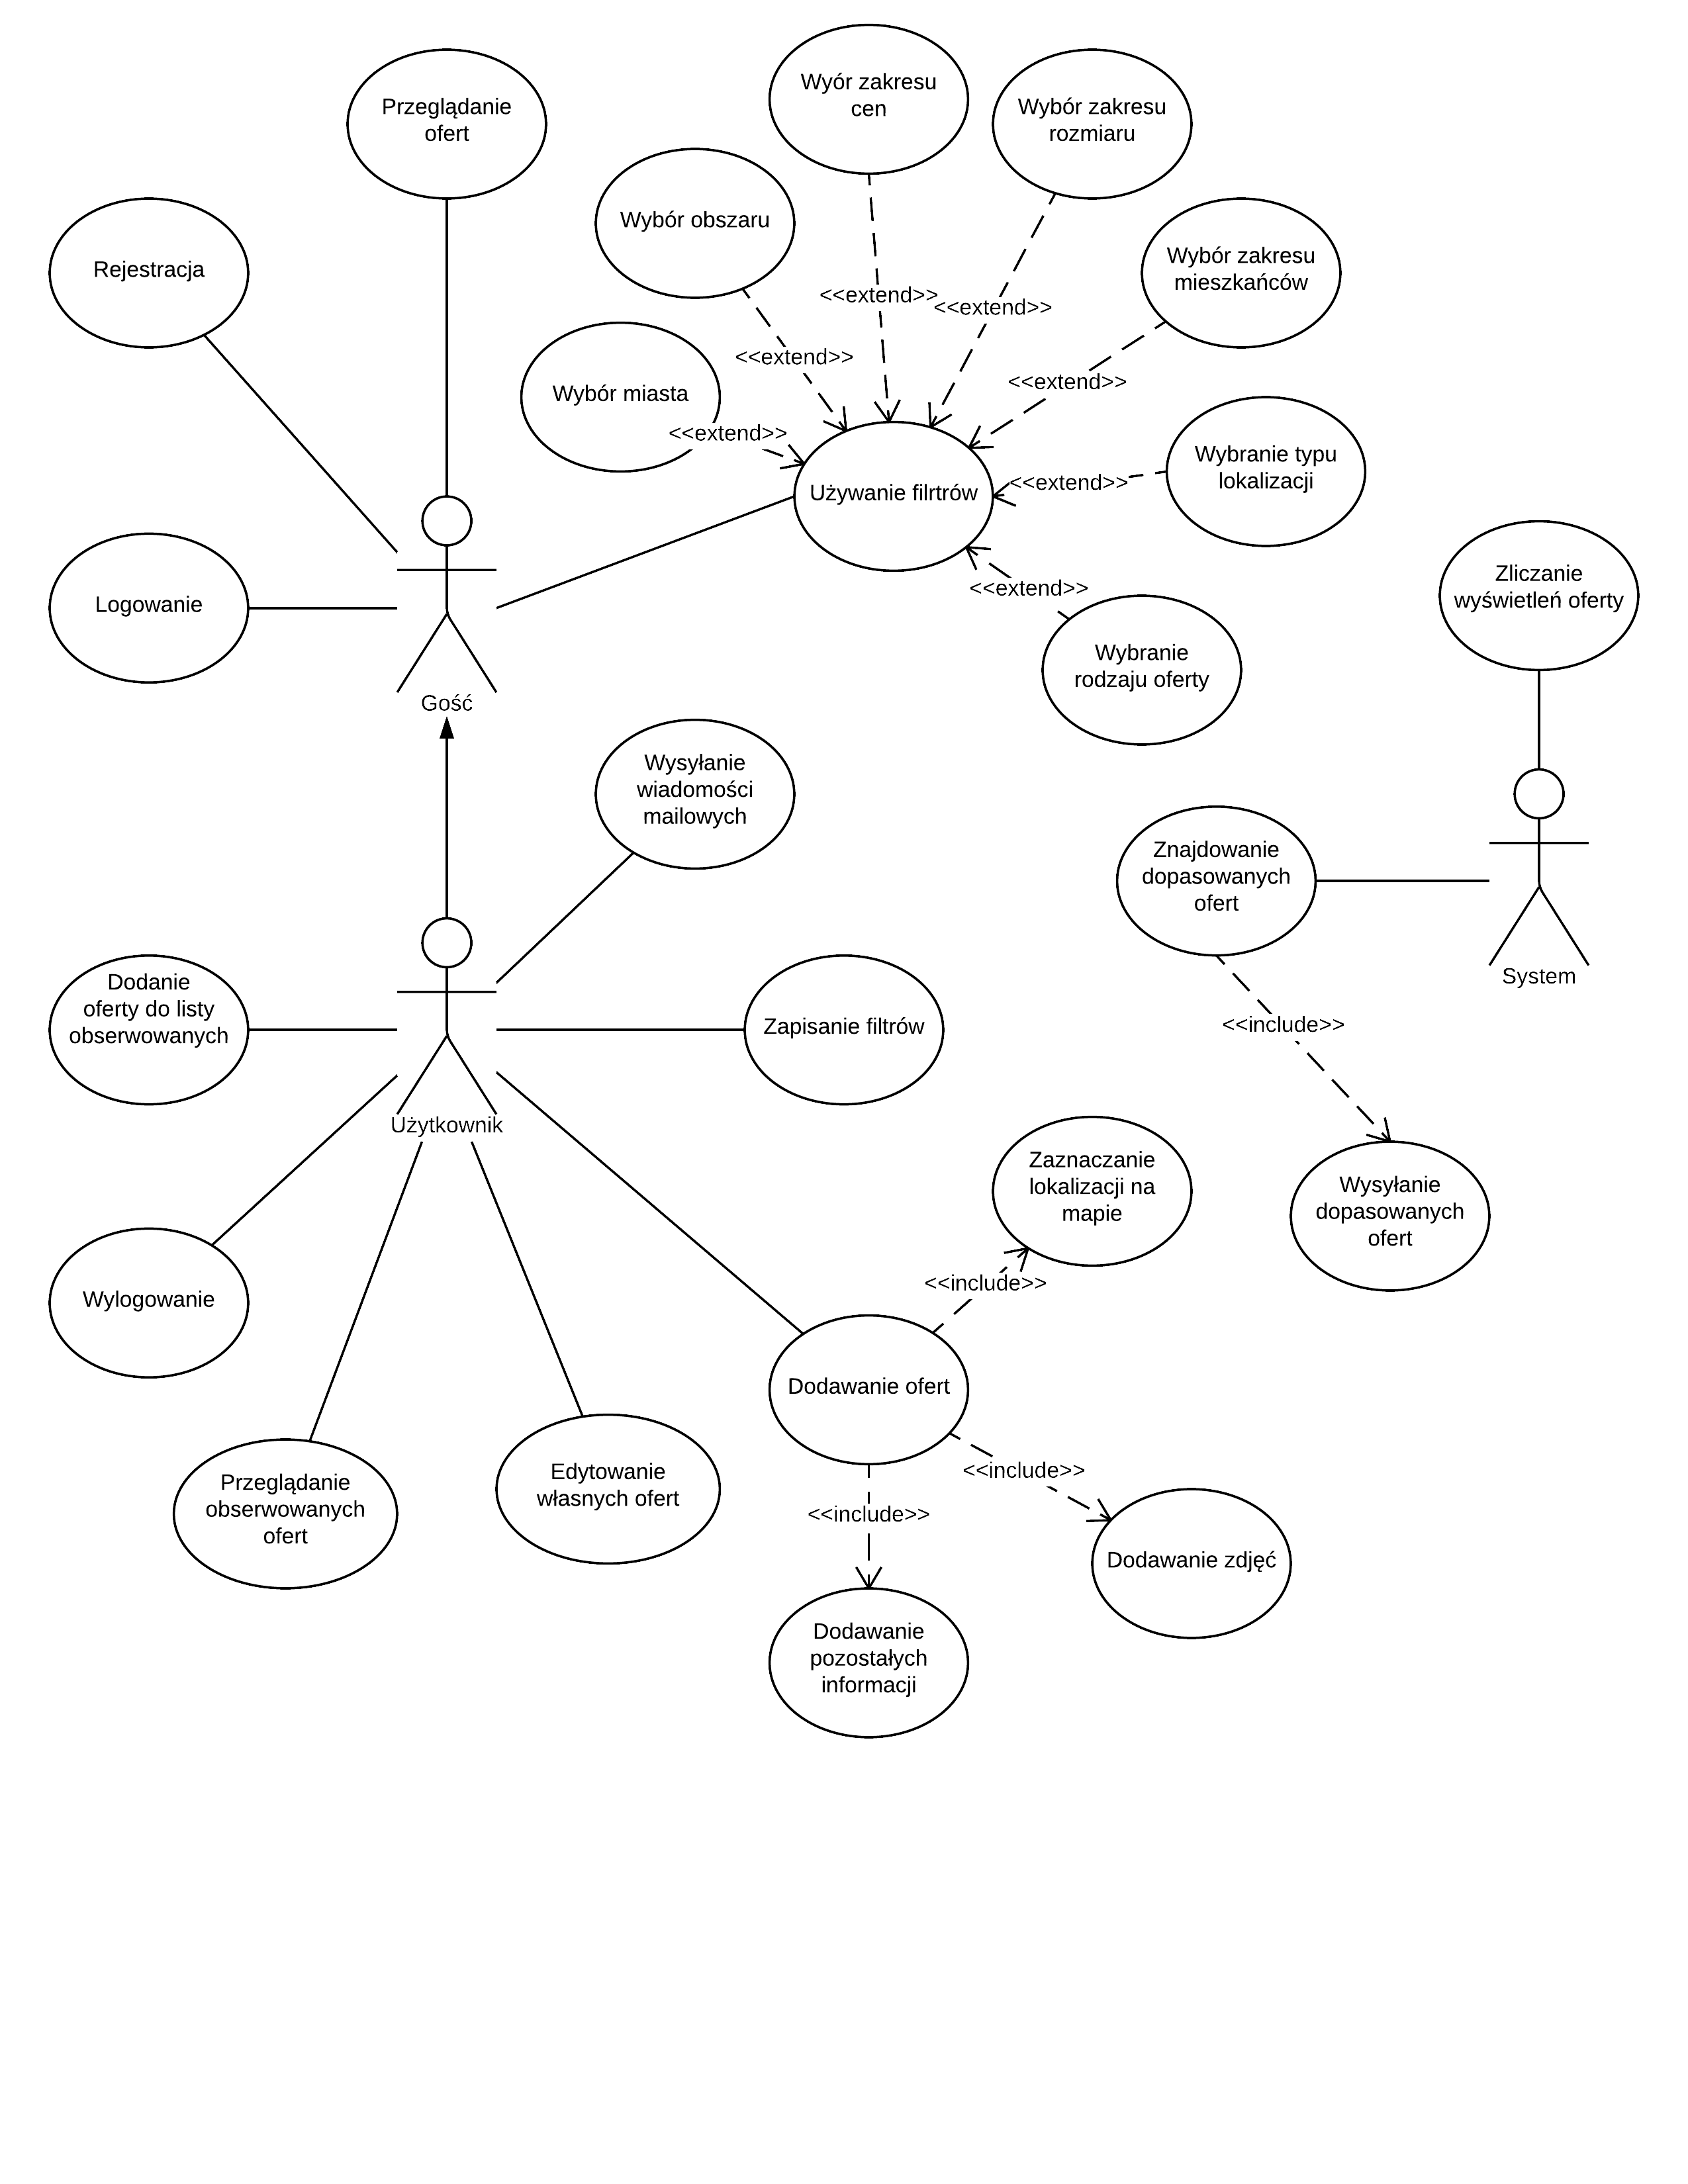
\includegraphics[keepaspectratio=true,scale=0.75]{pictures/use-case.png}}
\captionof{figure}{Diagram przypadków użycia}\label{use-case}
\end{minipage}

\section{Zidentyfikowanie obiektów świata rzeczywistego}
Poparawna identyfikacja obiektów świata rzeczywistego jest niezbędna do stworzenia poprawnego schematu bazy danych. Obiekty, które zostały zidentyfikowane podczas procesu analizy aplikacji to:
\begin{itemize}
\item Użytkownik (user)
\item Oferta (offer)
\item Zdjęcie (photo)
\item Lokalizacja (location)
\item Filtr (filter)
\end{itemize}
Zależności jakie zachodzą pomiędzy obiektami:\\
\noindent
\begin{minipage}{\linewidth}
\makebox[\linewidth]{
  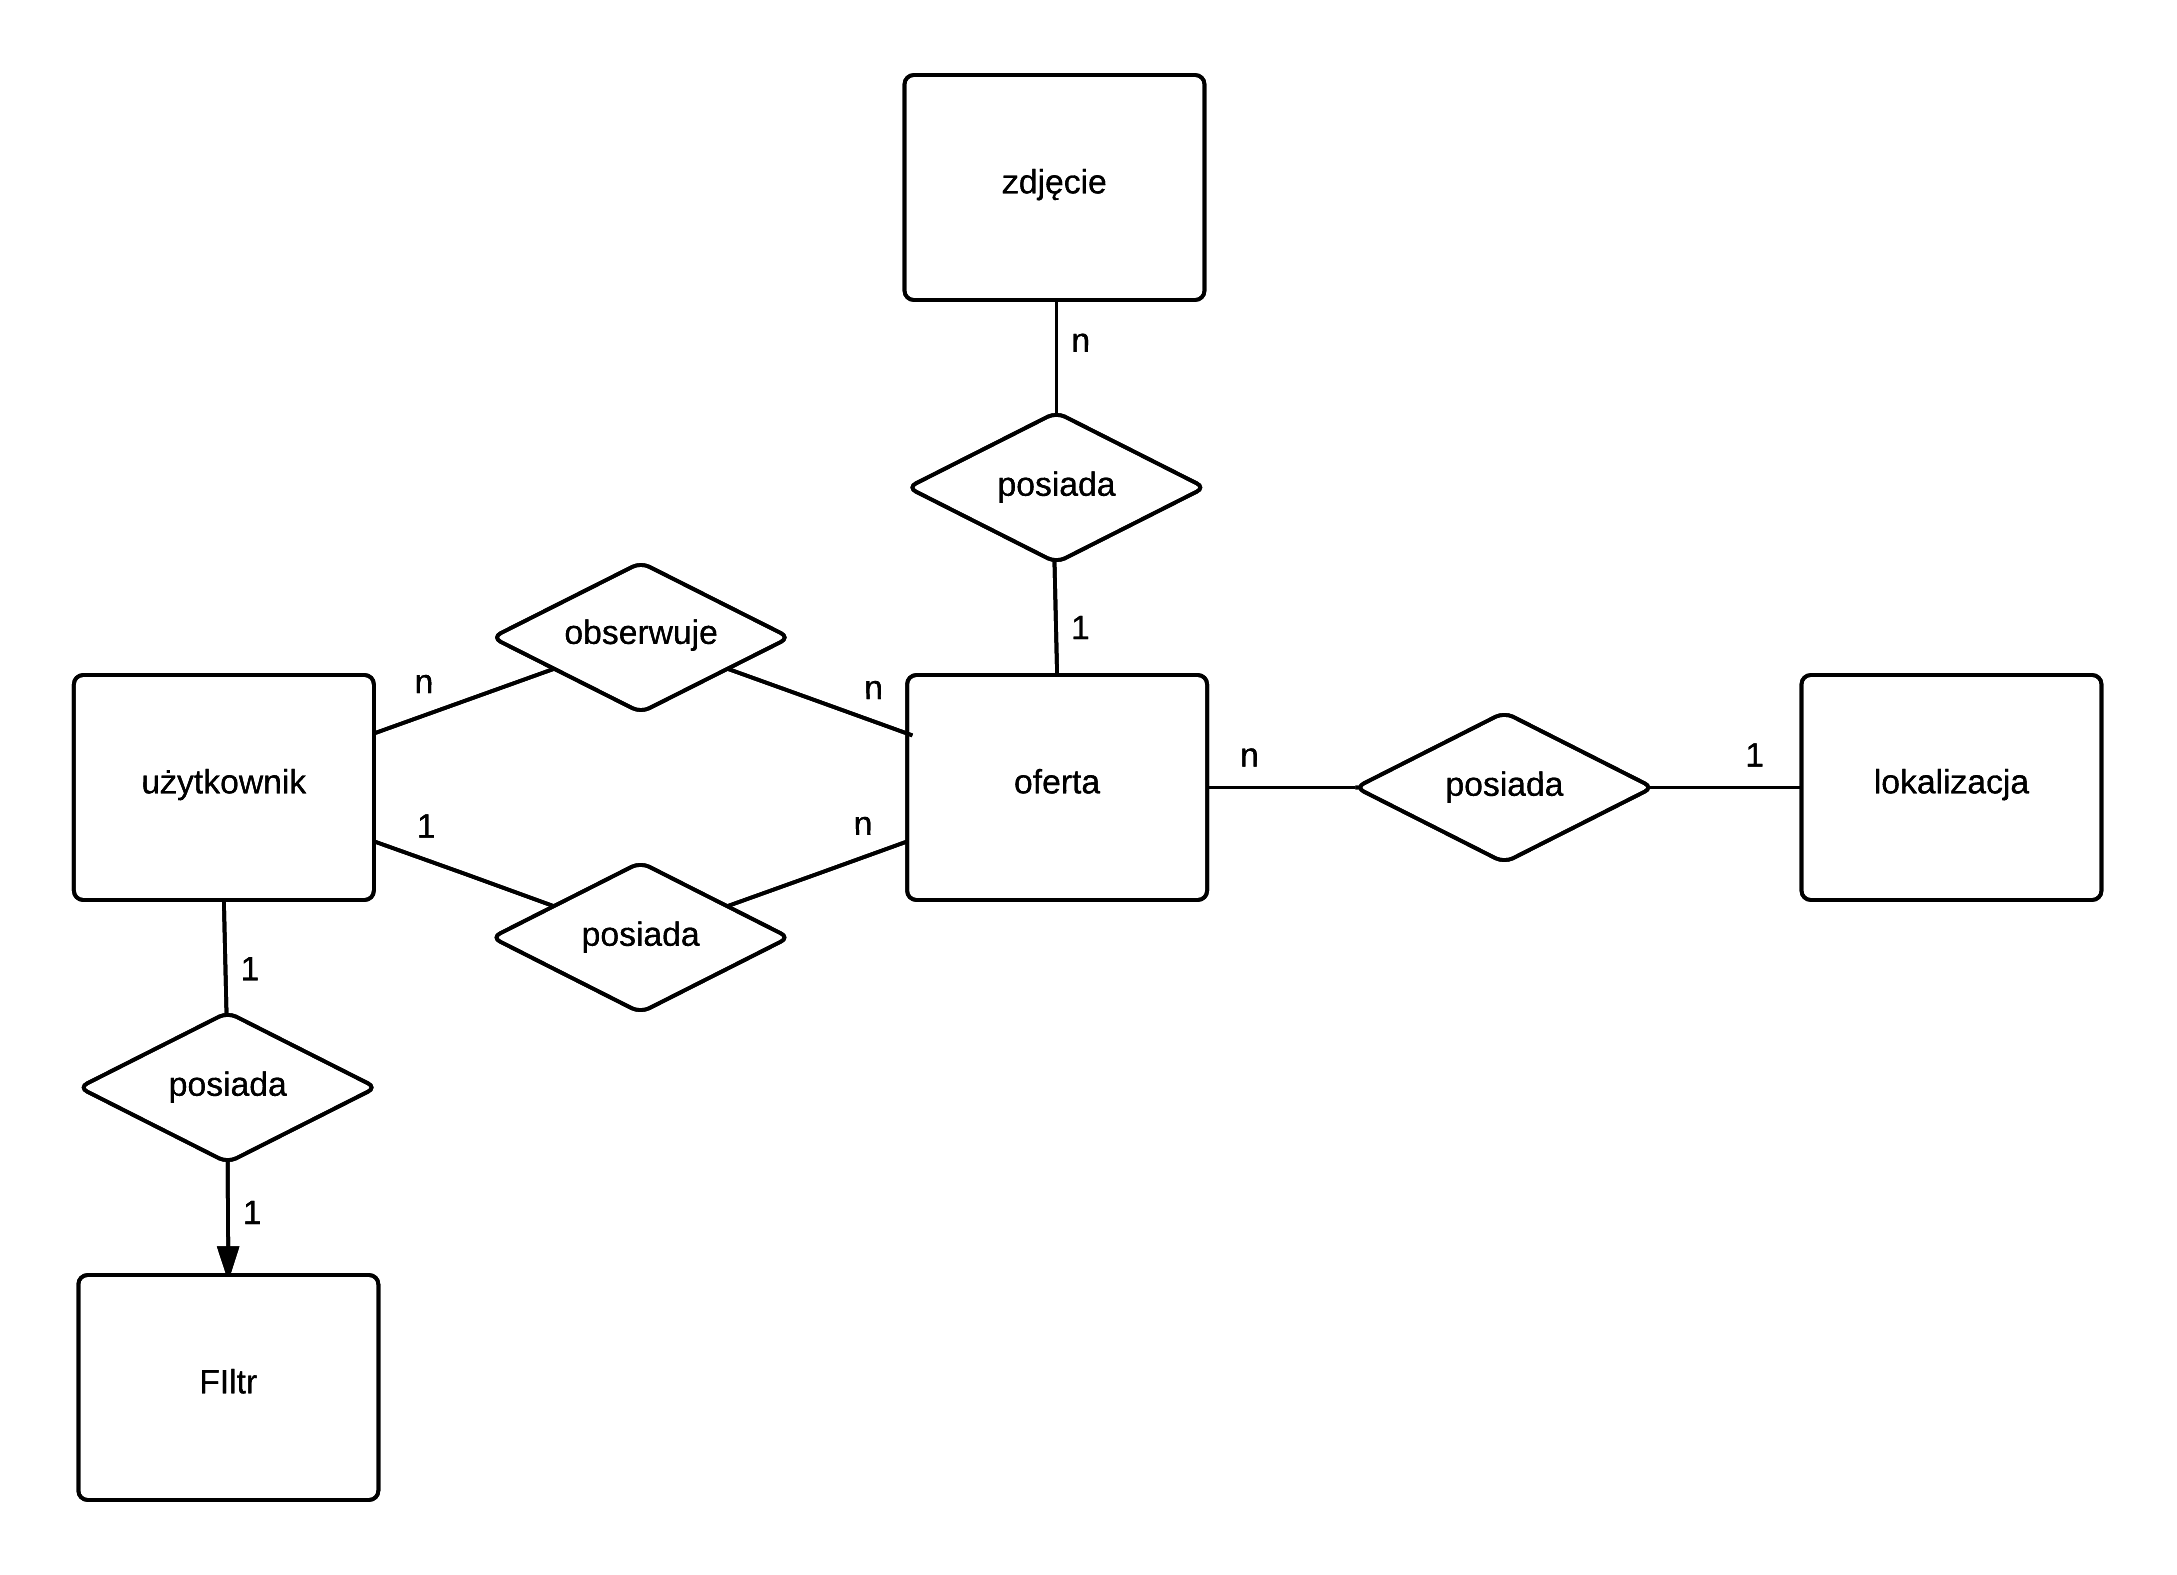
\includegraphics[keepaspectratio=true,scale=0.85]{pictures/erd.png}}
\captionof{figure}{Diagram ERD relacji pomiędzy encjami}\label{use-case}
\end{minipage}

\chapter{Projekt systemu}
\label{cha:analizaAplikacji}

\section{Architektura systemu}
\label{sec:architektura}
Architetura aplikacji jest typowa dla frameworku Ruby on Rails. Żądania od klienta są kierowane do serwera aplikacyjnego. Serwer kieruje żądania użytkowników do dyspozytora który przekierowuje żądanie do odpowiedniego kontrolera. Kontroler korzystając z mechanizmu ActiveRecord, który jest odpowiedzialny za mapowanie obiektów z bazą danych, otrzymuje konkretne dane. Następnie kontroler może przekierować żądanie oraz dane do innego kontrolera lub wysłać odpowiedź do użytkownika poprzez wyrenderowanie odpowiedzi w przeglądarce klienta lub poprzez moduł ActionMailer, który jest odpowiedzialny za wysyłanie wiadomości mailowych. Zadania które mają się wykonywać w tle trafiają do modułu ActiveJob, który jest odpowiedzialny za odpowiednie zakolejkowanie zadań i wywołanie ich w odpowiednim czasie.
\noindent
\begin{minipage}{\linewidth}
\makebox[\linewidth]{
  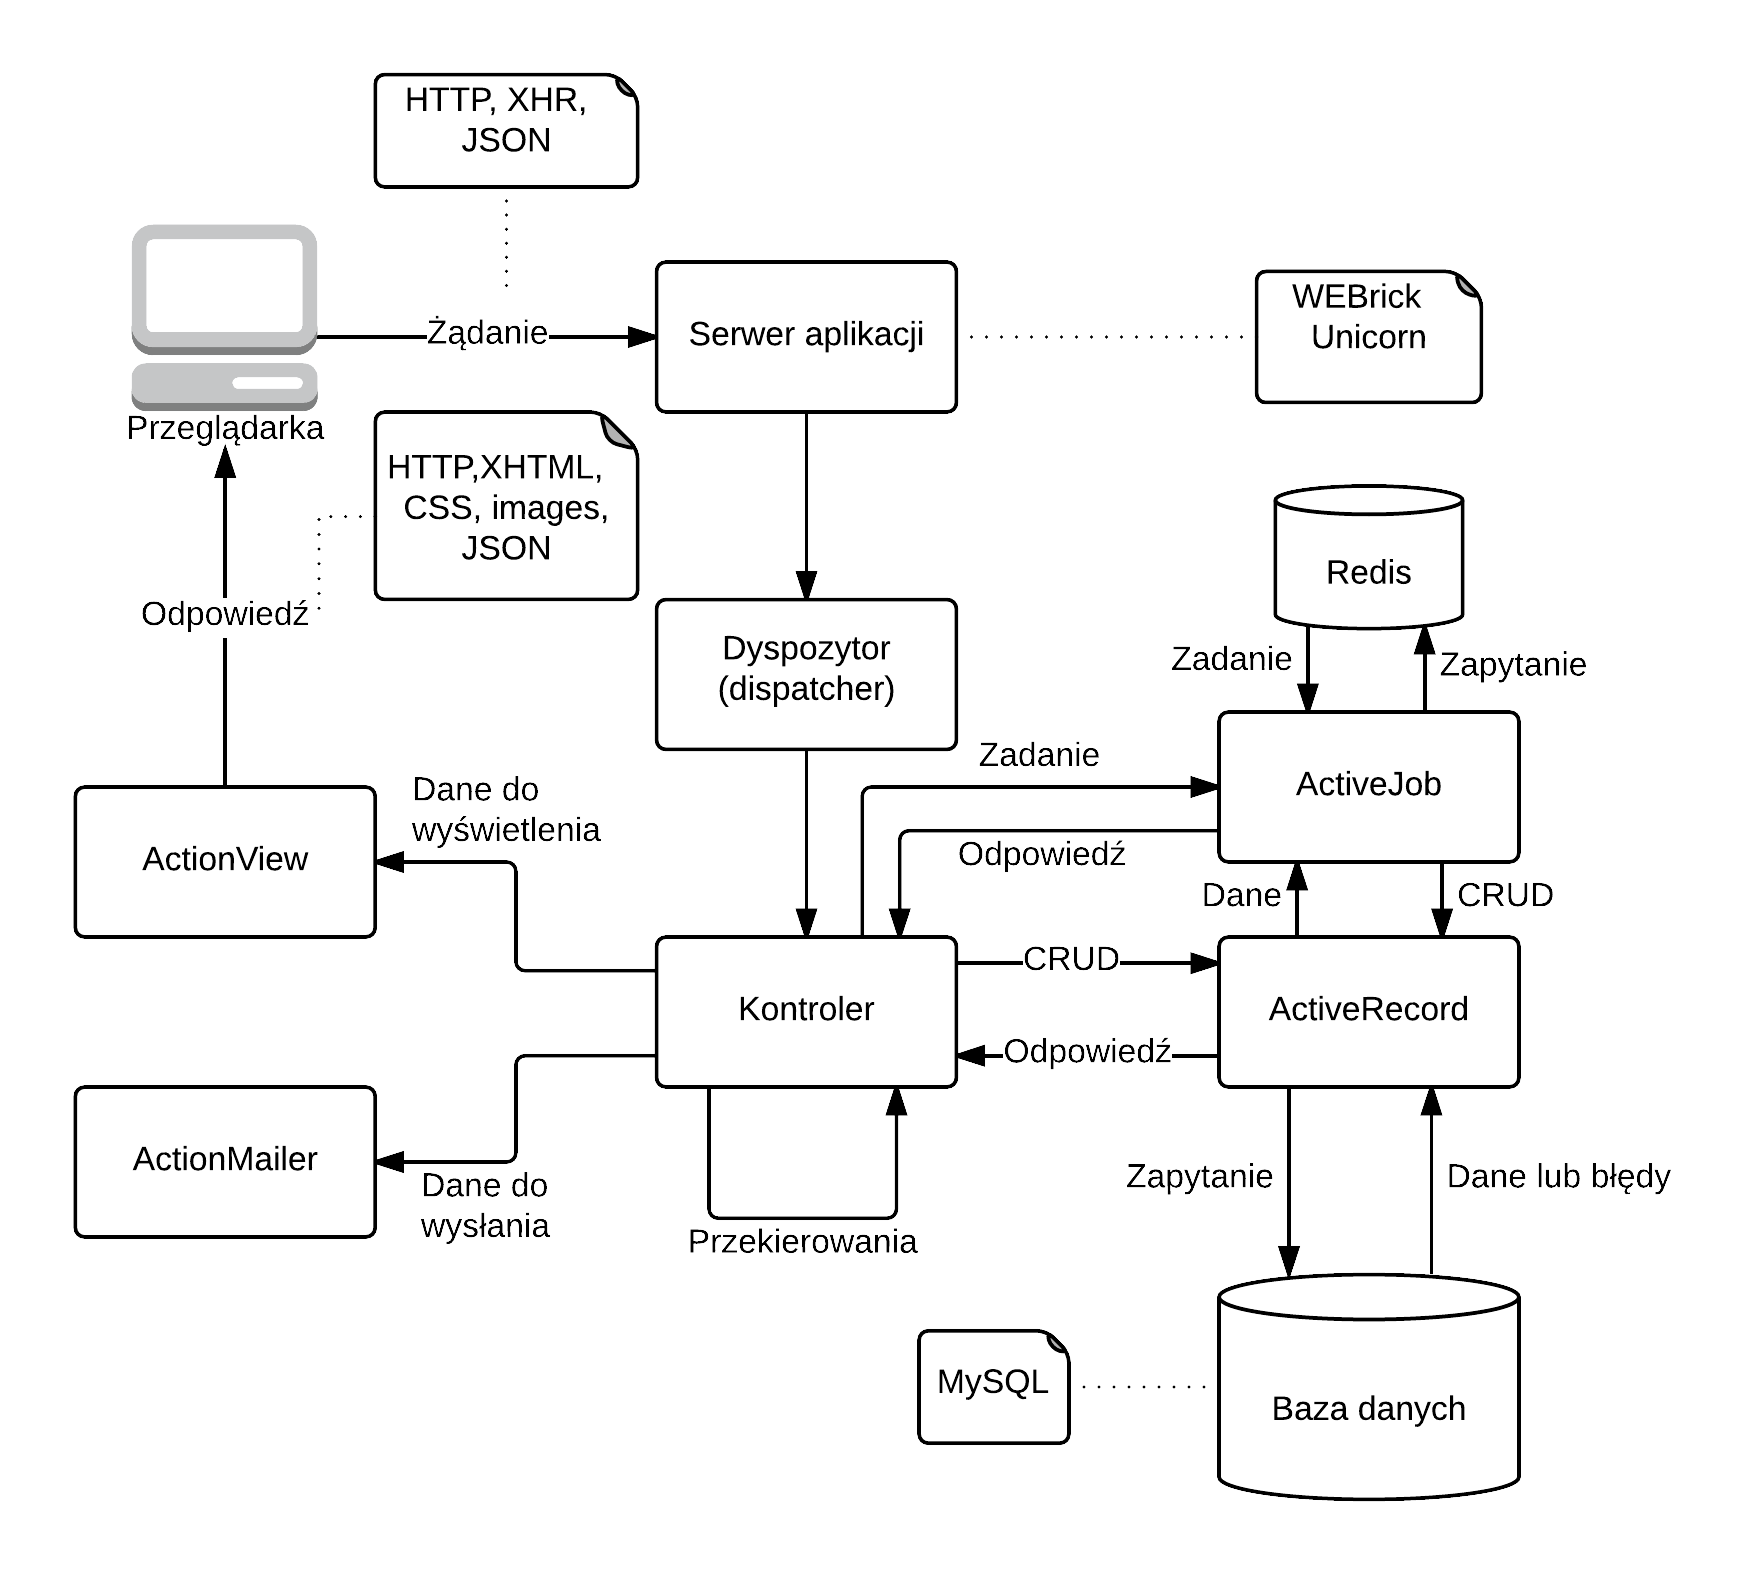
\includegraphics[keepaspectratio=true,scale=0.8]{pictures/architecture.png}}
\captionof{figure}{Diagram architektury}\label{use-case}
\end{minipage}

\section{Model bazy danych}
\label{sec;modelBazyDanych}
\noindent
\begin{minipage}{\linewidth}
\makebox[\linewidth]{
  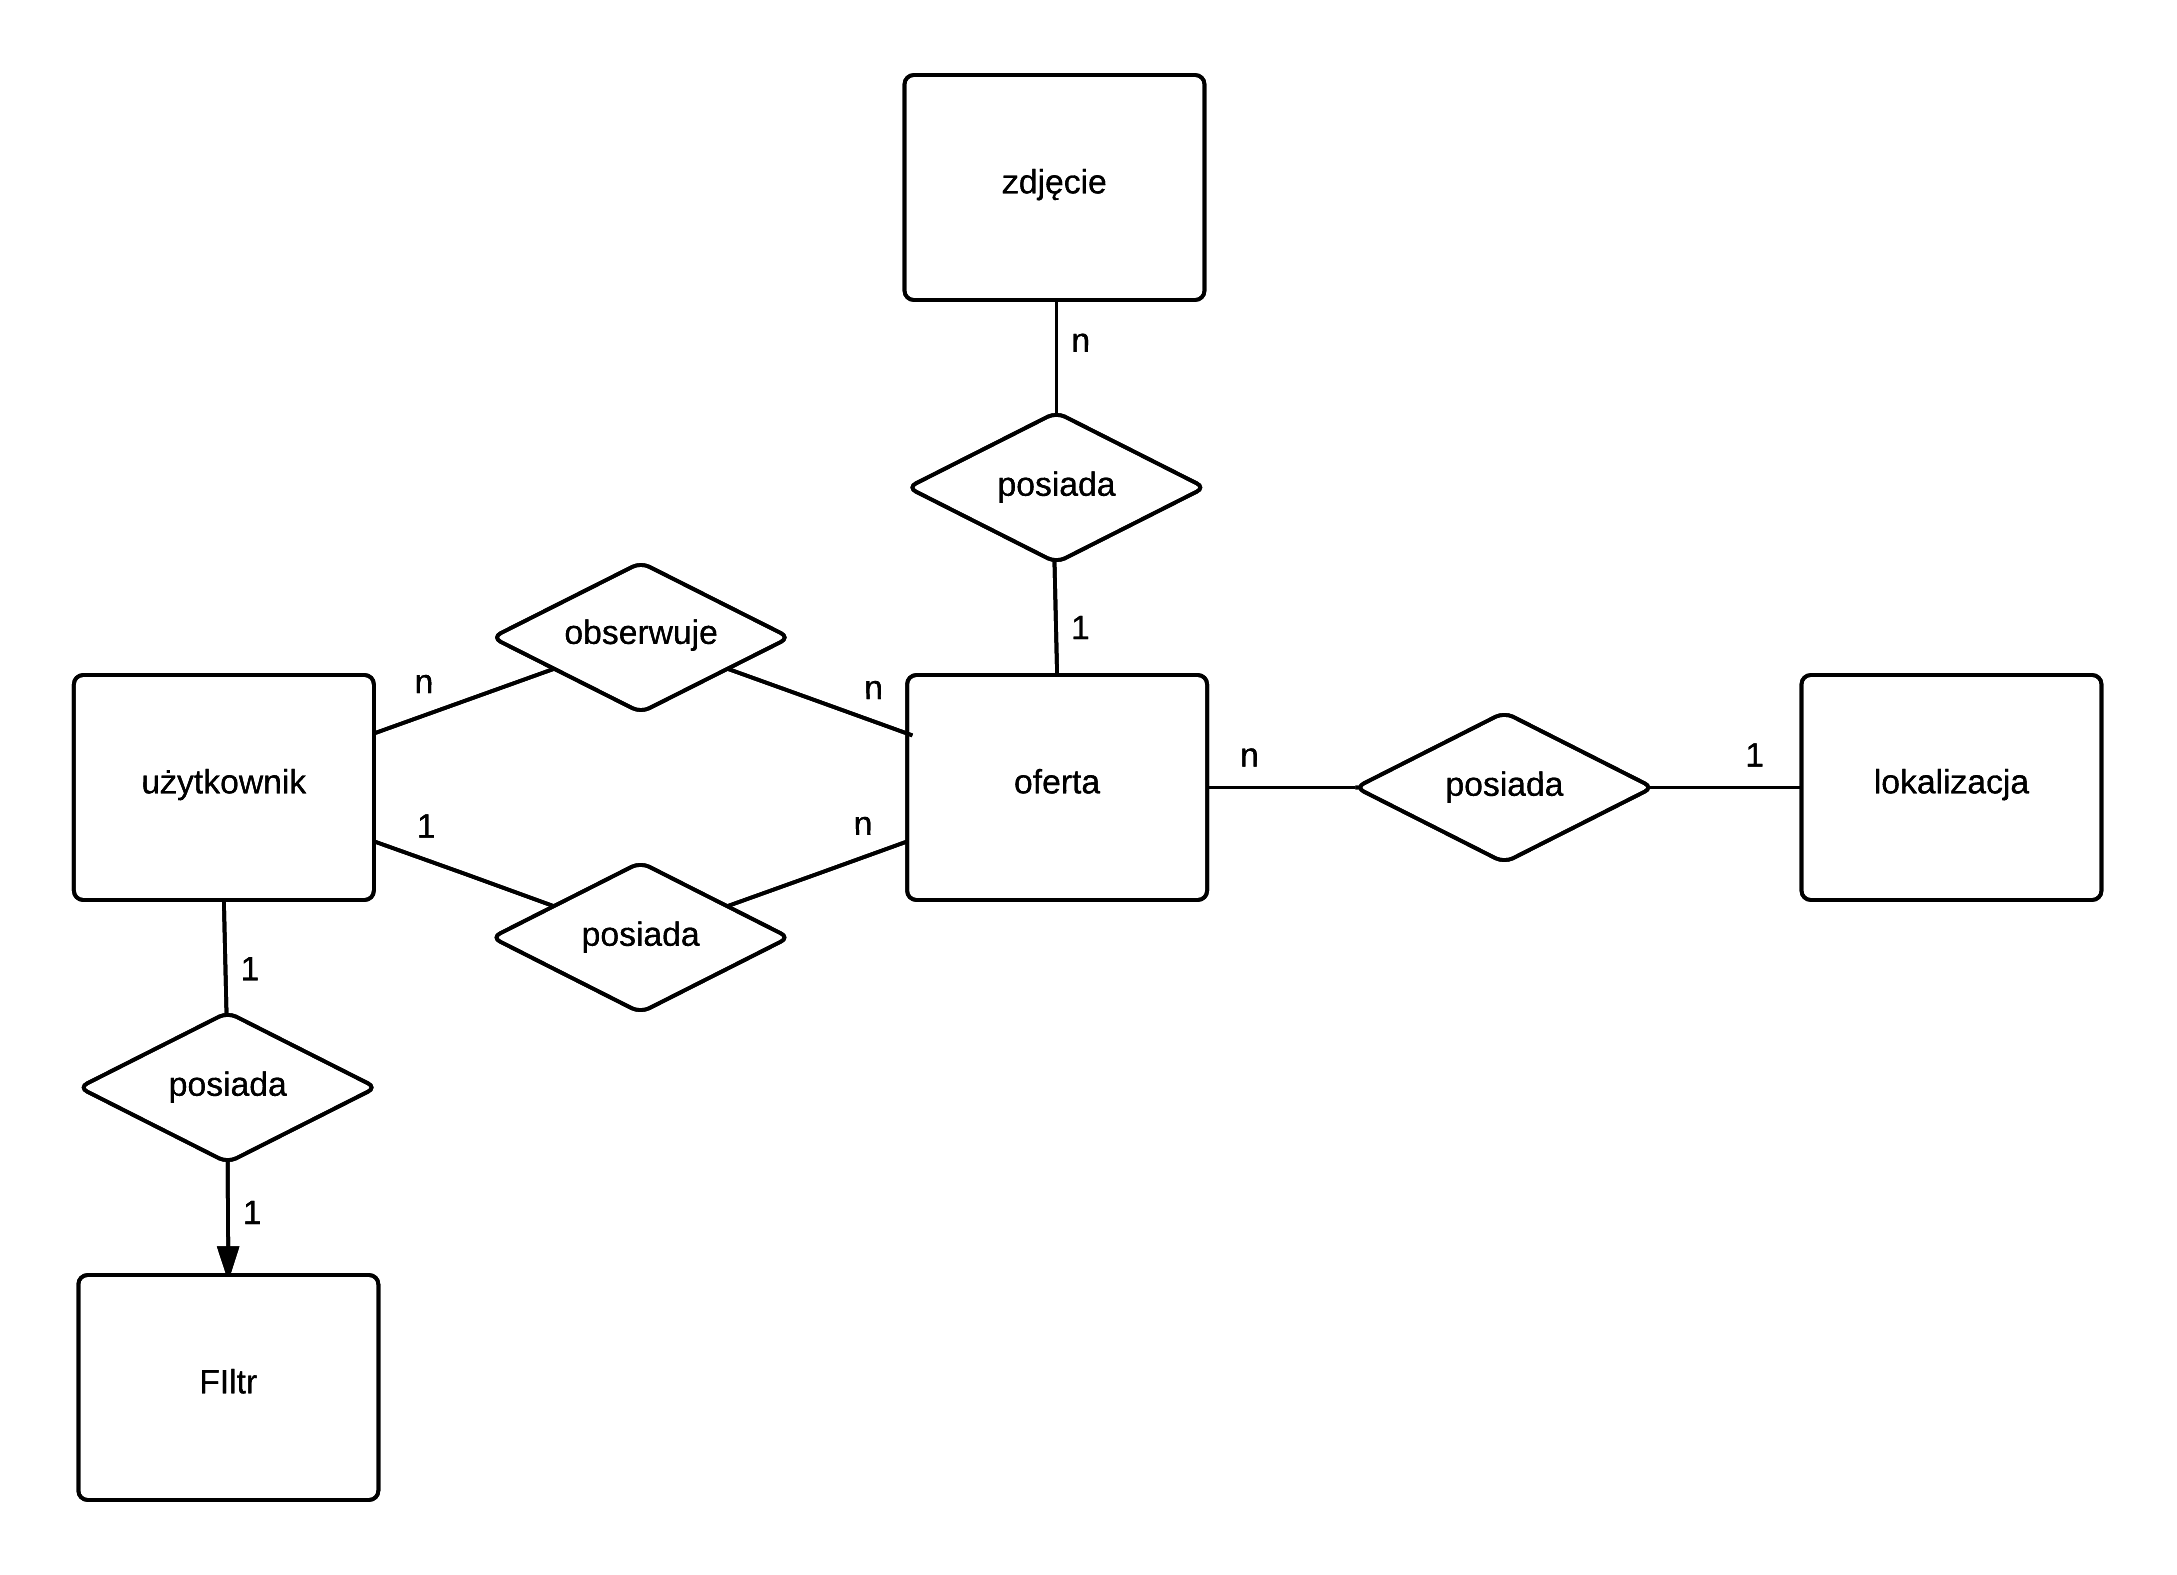
\includegraphics[keepaspectratio=true,scale=0.9]{pictures/erd.png}}
\captionof{figure}{Diagram ERD bazy danych}
\end{minipage}

\section{Interfejs graficzny}
\label{sec:interfejsGraficzny}
Strona graficzna aplikacji jest utrzymana w konwencji charakterystycznej dla aplikacji typu Single Page Application. Konwencja ta polega na umieszczeniu całej aplikacji oraz wszystkich funkcjonalności na jednej stronie interentowej w celu wywołania u użytkownika odczucia płynnego działania aplikacji podobnego do zwykłych aplikacji komputerowych. W technice tej cały potrzebny kod aplikacji (kod HTML, arkusze stylów CSS, skrypty JavaScript) jest pobierany podczas pierwszego załadowania aplikacji. Potrzebne elementy są dołączane dynamicznie do już załadowanej strony zazwyczaj jako odpowiedź na wywowałanie akcji przez użytkownika. Techniką która umożliwia dynamiczne generowanie treści strony jest dzięki bibliotece JavaScript jQury. Biblioteka ta umożliwa wykorzystanie XMLHttpRequest ze skryptów JavaScript. Żądania i odpowiedzi mogą być przesyłane bez konieczności przeładowywania strony. Każde wywołanie akcji przez użytkownika skutkuje wyświetleniem dodatkowego okna na stronie umożliwiającym wykonanie akcji, np. logowania, rejestracji.(Flanagan, David, "JavaScript - The Definitive Guide", 5th ed., O'Reilly, Sebastopol, CA, 2006, p.497)

Zazwyczaj oferty w serwisach ogłoszeniowych są wyświetlane jako lista. Jest to dosyć niewygodne podejście gdyż, użytkownik nie może zbyt szybko ocenić czy dane ogłoszenie jest dla niego interesujące. W opisywanej aplikacji zdecydowano się na zaimplementowanie zupełnie odmiennego sposobu prezentacji ofert. Ofety są prezentowane jako znaczniki na mapie dzięki czemu, każde ogłoszenie jest nierozerwalnie związane z lokalizacją. Zarówno znaczniki jak i mapa pochodzą z Google Maps API. W celu filtrowania dostępnych ofert aplikacja dostarcza zestaw filtrów, którymi użytkownik może swobodnie manipulować. 

\section{Interfejs restowy}
\label{sec:interfejsRestowy}

\section{Opis struktury danych oferty}
\label{sec:strukturaOferty}
Kluczową strukturą dla poprawnego działania całego programu jest struktura oferty. Jest to bardzo rozbudowany model, lecz było to konieczne ze względu na dużą liczbę atrubutów którymi oferty muszą być opisane. Atrybuty oferty można podzielić ze względu na typ:
\begin{itemize}
\item Numeryczny całkowity
\begin{itemize}
\item size - rozmiar mieszkania w metrach kwadratowych
\item rooms - liczba pokoi
\item people - liczba osób mogących mieszkać w danej lokalizacji
\item floor - piętro budynko
\item views - liczba wyświetleń oferty
\end{itemize}
\item Znakowy
\begin{itemize}
\item offer\_type - typ oferty
\begin{itemize}
\item O - od właściciela
\item A - od agencji mieszkaniowej
\end{itemize}
\item location\_type - typ lokalizacji 
\begin{itemize}
\item H - dom
\item F - mieszkanie
\item R - pokój
\end{itemize}
\item building\_type - typ budynku
\begin{itemize}
\item H - dom
\item T - kamienica
\item A - blok
\end{itemize}
\item parking\_type - typ parkingu
\begin{itemize}
\item N - brak możliwości zaparkowania auta
\item R - istnieje możliwość ale miejsce nie jest gwarantowane
\item O - miejsce gwarantowane niezadaszone
\item G - miejsce w garażu
\end{itemize} 
\item heating\_type - typ ogrzewania
\begin{itemize}
\item G - gazowe
\item E - elektryczne
\item C - Centralne - opał stały
\item D - ogrzewanie miejskie
\end{itemize}
\end{itemize}
\item Numeryczny niecałkowity
\begin{itemize}
\item parking\_price - cena za parking
\item media\_price - opłata za wodę, prąd, internet itd.
\item rent\_price - kwota odstępnego dla właściciela 
\item sum\_price - kwota całkowita
\item bail - kaucja
\end{itemize}
\item Logiczny
\begin{itemize}
\item animals - czy są dozwolone zwierzęta
\item students - czy osoby wynajmujące mogą być studentami
\item basement - czy nieruchomość posiada piwnicę
\item balcony - czy nieruchomość posiada balkon
\item elevator - czy w budynku jest winda
\item internet - czy jest dostępny internet w mieszkaniu
\item cigaretts - czy w mieszkaniu można palić tytoń
\end{itemize}
\item Data
\begin{itemize}
\item from - od kiedy nieruchomość jest dostępna
\end{itemize}
\end{itemize} 
Można również zauważyć, że oferta posiada klucz obcy do tabeli locations. Tabela locations zawiera podstawowe dane adresowe. Zastosowana została tutaj relacja jeden do jednego w celu ograniczenia rozmiaru tabeli offers oraz rozgraniczenia logicznego modeli.\\
Równie obszerny model to tabela filters. Nie zostanie jednak omówione w pracy jej atrybuty, gdyż są bardzo podobne do atrybutów modelu offers.

\chapter{Opis implementacji}
\label{cha:uzywaneTechnologie}

\section{Opis użytych technologii i narzędzi}
\label{sec:technology}
Przy implementacji pracy zostały użyte następujące technologie i narzędzia:
\begin{itemize}
\item Ruby on Rails - jest to framework webowy służący do tworzenia aplikacji internetowych. Został napisany w interpretowanym skryptowym języku Ruby. Ruby on Rails wpisuje się w architekturę Model View Controller (MVC), dostarczając podstawowe struktury dla bazy danych, serwisów oraz stron internetowych. Domyślnym formatem wymiany danych w tym frameworku jest JSON oraz XML. Przy wyświetlaniu stron zaleca się korzystanie z szablonów ERB lub HAML, JavaScript oraz SASS ( jest to język podobny do CSS cechujący się znacznie większą przejrzystością oraz mniejszą ilością kodu). Ruby on Rails w bardzo prosty sposób umożliwa dołączenie do aplikacji dodatkowych, gotowych bibliotek nazywanych gemami. Nadrzędnym celem twórców tego frameworku było wprowadzenie zasad DRY (Don't repeat yourself - Nie powtarzaj się) oraz CoC (Convention over Configuration - konwencja ponad konfiguracją). Dzięki kierowania się tymi zasadami kod, który powstaje podczas pisania aplikacji cechuję się wysoką  przejrzystością oraz zwięzłością.\cite{rails}
\item Javascript + JQuery + Google Maps API - Javascript to skryptowy język programowania stworzony pod koniec lat 90. ubiegłego wieku przez firmę Netscape. Język ten znacząco rozszerza możliwości stron internetowych, poprzez przeniesienie części niezbyt wrażliwych funkcjonalności na przeglądrkę użytkownika. Dzięki temu możliwe jest odciążenie serwerów, które w przeciwnym razie musiały się zajmować np. walidacją formularzy. Dzieki JavaScript oraz biblioteki JQuery, możliwe jest uzyskanie wrażenia responsywności danej strony internetowej. 
Google Maps API to biblioteka stworzona w języku JavaScript przez Google. Jest to zbiór funkcji, które umożliwiają wyświetlenia mapy oraz dostarczają możliwości manipulowania nią. Korzystanie z niej w okrojonej wersji jest całkowicie darmowe tylko dla stron internetowych, które nie pobierają opłat od użytkowników za korzystanie z nich.\\
 Pomimo dużej ilości gotowych frameworków umożliwiających szybkie tworzenie strony w Javascript, autor zdecydował się na stworzenie własnego prostego frameworka, który umożliwa wykorzystywanie tych samych elementów w celu szybszego tworzenia widoków.
\item RubyMine IDE - jest to środowisko służące do tworzenia oprogramowania w języku Ruby stworzone przez firmę JetBrains. Środowisko te udostępnia szeroką gammę narzędzi np. automatyczne zarządzanie bibliotekami, graficzny debugger, dostęp do bazy danych. Narzędzie wspiera również popularne technologie wykorzystywane przy pracy z językiem Ruby takie jak: Bundler, RSpec, Capistrano, Git. RubyMine został  stworzony w oparciu o IntelliJ IDEA - zintegrowane środowisko programistyczne do tworzenia aplikacji w języku Java. Korzystanie z programu jest oparte o płatną licencję, którą można otrzymać bezpłatnie w ramach specjalnego programu skierowanego do studentów uczelni na całym świecie.
\end{itemize}

\section{Autoryzacja i autentykacja}
\label{sec:autoryzacjaAutentykacja}
Zabezpieczeniem aplikacji w Ruby on Rails zazwyczaj zajmuje się gem devise. Jest to biblioteka, która umożliwia np. bezpieczene przechowywanie haseł\cite{rails}. W pracy nie zastosowano jednak tego rozwiązania, gdyż autor chciał mieć pełną  kontrolę nad przesyłaniem i odpowiednim przechowywaniu haseł.\\
Autentykacja jest przeprowadzona za pomocą hasła podanego przez użytkownika przy rejestracji. Hasło to jest szyfrowane dwukrotnie za pomocą algorytmu SHA1. Szyfrowanie dwukrotne jest dodatkowym utrudnieniem przy próbie rozszyfrowania hasła oraz powoduje, że hasło wykradzione z bazy danych jest bezużyteczne.\\
\begin{minipage}{\linewidth}
\makebox[\linewidth]{
  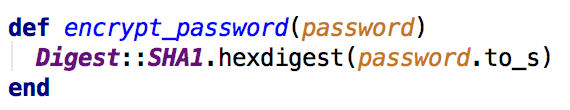
\includegraphics[keepaspectratio=true,scale=0.85]{pictures/encryptpassword.png}}
\captionof{figure}{Szyfrowanie hasła}\label{encryptpassword}
\end{minipage}\\
Autoryzacja ma za zadanie zweryfikować czy dany użytkownik faktycznie ma dostęp do żądanych zasobów. W aplikacji zostało to zrealizowane za pomocą  metody sprawdzającej czy dane o które zapytanie wysłał użytkownik naprawdę do niego należą. Dzieje się to dzięki sprawdzania wartości tokenu, który jest generowany dla każdego użytkownika. Token ten jest unikalny dla każdego użytkownika a jego czas życia ogranicza się do długości sesji. 
\begin{minipage}{\linewidth}
\makebox[\linewidth]{
  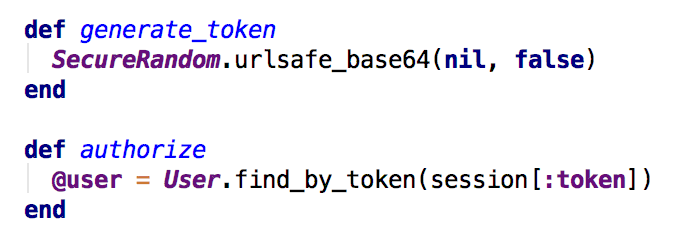
\includegraphics[keepaspectratio=true,scale=0.85]{pictures/authorization.png}}
\captionof{figure}{Autoryzacja za pomocą tokenu}\label{authorization}
\end{minipage}\\
Weryfikacja odbywa się przy każdej metodzie wskazanej w adnotacji before\_action:\\
\begin{minipage}{\linewidth}
\makebox[\linewidth]{
  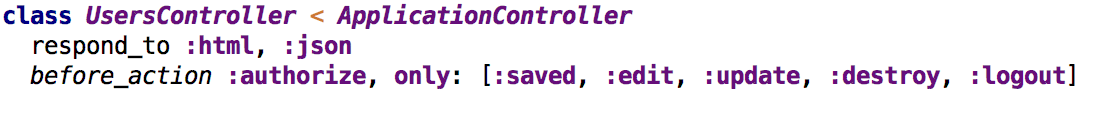
\includegraphics[keepaspectratio=true,scale=0.85]{pictures/beforeaction.png}}
\captionof{figure}{Wskazanie metod, które będą autoryzowane}\label{before_authorization}
\end{minipage}

\chapter{Podręcznik użytkownika}
\label{cha:podrecznik uzytkownika}

\section{Rejestracja}
\label{sec:rejestracja}

\section{Logowanie}
\label{sec:logowanie}

\section{Dodanie oferty}

\section{Edycja oferty}

\section{Usunięcie oferty}

\section{Filtrowanie wyników}

\section{Dodanie oferty do obserwowanych}
\chapter{Testy systemu}
\label{cha;testySystemu}

Zostały przeprowadzone manualne testy aplikacyjne, które zweryfikowały czy powstała aplikacja spełnia postawione mu wymagania. Oprócz testów manualnych zostały wykonane również testy behawioralne napisane we frameworku RSpec. Testy behawioralne zostały napisane zgodnie z metodyką  TDD (Test Driven Development). Wymagania, które zostały przetestowane na działającym serwisie to:
\begin{itemize}
\item Niezawodność
\item Intuicyjność interfejsu
\item Bezpieczeństwo danych
\item Odporność na nieautoryzowany dostęp do danych
\end{itemize}
Oprócz sprawdzenia czy system spełnia postawione przed nim wymagania, przetestowane zostały również funkcjonalności wyspecyfikowane w rozdziale 2. \textit{Analiza wymagań}

\section{Scenariusze testowania}
Najważniejsze funkcjonalności systemu były przetestowane wzorując się na poniższych scenariuszach:
 \begin{enumerate}
 \item Rejestracja
 \begin{itemize}
 \item Warunki początkowe:
 \begin{itemize}
 \item W sesji przeglądarki nie znajduję się sesja należąca do żadnego użytkownika
 \end{itemize}
 \item Kroki testowe:
 \begin{enumerate}
 \item Naciśnięcie przycisku \textbf{Registration} - w odpowiedzi powinno pojawić się dodatkowe okno z formularzem rejestracji.
 \item Wprowadzenie niepoprawnych danych takich jak:
 \begin{itemize}
 \item Brak któregokolwiek z atrybutów formularza
 \item Niepoprawny adres mailowy
 \item Adres mailowy jest już wykorzystany
 \item Zbyt krótkie hasło
 \end{itemize}
 Spowoduje błąd walidacji formularza w skutek czego, użytkownik zostanie poinformowany o przyczynie niepowodzenia. Pola formularza oprócz hasła powinny pozostać niezmienione.
 \item Wprowadzenie poprawnych danych skutkuje utworzeniem profilu użytkowniku w aplikacji oraz automatycznym zalogowanie użytkownika do aplikacji.
 \end{enumerate}
 \end{itemize}

 \item Logowanie 
  \begin{itemize}
   \item Warunki początkowe:
    \begin{itemize}
     \item W sesji przeglądarki nie znajduje się sesja należąca do żadnego użytkownika
     \item Istnieje co najmniej jeden profil użytkownika
    \end{itemize}
   \item Kroki testowe:
    \begin{enumerate}
     \item Naciśnięcie przyscisku \textbf{Login} - w odpowiedzi powinno pojawić się dodatkowe okno z formularzem logowania
     \item Wprowadzenie niepoprawnych danych takich jak:
      \begin{itemize}
       \item Brak adresu mailowego lub hasła
       \item Adres mailowy niewystępujacy w bazie danych
       \item Hasło nie pasujące do podanego adresu mailowego
      \end{itemize}
      Spowoduje błąd walidacji formularza, w skutek czego, użytkownik zostanie poinformowany o przyczynie niepowodzenia. Pole adresu mailowego powinno zostać niezmienione.
     \item Wprowadzenie poprawnych danych skutkuje zalogowaniem użytkownika dla aplikacji oraz dodaniem do ciasteczek obiektu z informacją o sesji użytkownika.
    \end{enumerate}
  \end{itemize}

 \item Dodawanie oferty
  \begin{itemize}
   \item Warunki poczatkowe:
    \begin{itemize}
     \item Użytkownik jest zalogowany do systemu
    \end{itemize}
   \item Kroki testowe:
    \begin{enumerate}
     \item Naciśnięciu przycisku \textbf{Add offer} - w odpowiedzi powinno pojawić się dodatkowe okno z formularzem tworzenia nowej oferty
     \item Wprowadzenie nieporawnych danych spowoduje błąd walidacji oraz wyświetlenie odpowiednich komunikatów o przyczynie niepowodzenia walidacji
     \item Wprowadzenie poprawnych danych oraz naciśnięcie przycisku \textbf{Submit} powoduje przejście do następnego okna zawierającego formularz dodawania zdjęć.
     \item Wybranie przycisku dodawania zdjęcia powinno otworzyć okno z systemową przeglądarką plików.
     \item Naciśnięcie przycisku \textbf{Submit} spowoduje próbę zapisu zdjęcia - jeżeli format pliku nie należy do obsługiwanych przez aplikację, zdjęcie nie zostanie dodane. W przeciwnym wypadku zapis zdjęcia zakończy się powodzeniem oraz przejściem do formularza dodania lokalizacji.
     \item Wybranie przycisku \textbf{Create another} spowoduję zapisanie zdjęcia przy zachowaniu warunków podanych powyżej. Następnie wróci do formularza dodawnia zdjęcia, wyświetlając już dodane zdjęcia.
     \item W formularzu oferty należy zaznaczyć pozycję na mapie oraz podać dokładny adres w przeciwnym wypadku użytkownik powinien zostać poinformowany o przyczynach braku sukcesu po kliknięciu przycisku \textbf{Submit}
     \item Jeżeli wszystkie dane w formularzu lokalizacji są walidowalne, oferta powinna zostać utworzona. Na mapie powinien się natychmiast pojawić znacznik odpowiadający lokalizacji danej oferty.
    \end{enumerate}
  \end{itemize}

 \item Wyświetlanie oferty
  \begin{itemize}
   \item Warunki początkowe:
    \begin{itemize}
     \item W aplikacji istnieje co najmniej jedna oferta.
    \end{itemize}
   \item Kroki testowe:
    \begin{enumerate}
     \item Naciśnięcie znacznika na mapie reprezentującego ofertę
     \item Użytkownik powinien zaobserwować pojawienie się nowego okna wypełnionego danymi oferty
     \item Użytkownik do którego należy dane ogłoszenie powinien (będąc zalogowanym) widzieć opcję edycji ogłoszenia.
     \item Zalogowany użytkownik do którego nie należy dane ogłoszenie powinien mieć możliwość dodania oferty do obserwowanych ofert.
     \item Użytkownik zarejestrowany i niezarejestrowany powinien mieć możliwość zamknięcia oferty klikając na krzyżyk znajdujący się w prawym górnym rogu lub gdziekolwiek poza ofertą.
    \end{enumerate}
  \end{itemize} 

 \item Edycja oferty
  \begin{itemize}
   \item Warunki początkowe:
    \begin{itemize}
     \item Użytkownik jest zalogowany
     \item W aplikacji istnieje co najmniej jedna oferta przypisana dla zalogowanego użytkownika
    \end{itemize}
   \item Kroki testowe:
    \begin{enumerate}
     \item Naciśnięcie znacznika na mapie reprezentującego ofertę
     \item Użytkownik powinien zaobserwować pojawienie się nowego okna wypełnionego danymi oferty
     \item Użytkownik do którego należy dane ogłoszenie powinien (będąc zalogowanym) widzieć opcję edycji ogłoszenia. Po naciśnięciu tego przycisku powinno pojawić się okno z formularzem służącym do edytowania informacji o ofercie.
     \item Kliknięcie przycisku \textbf{Submit} w przypadku pozytywnej walidacji zapisuje zmiany i przenosi użytkownika do formularza edycji zdjęć. W przeciwnym wypadku użytkownik zostaje powiadomiony o przyczynie niepowodzenia walidacji.
     \item Użytkownik może dodać kolejne zdjęcia lub usunąć już istniejące za pomocą przycisku w kształcie litery \textbf{X}.
     \item Po skończeniu edycji użytkownik powinien zostać przeniesiony do formularza edycji lokalizacji.
     \item Po naciśnięciu przycisku \textbf{Submit} oferta powinna zostać zaktualizowana lub w przypadku niepoprawnej walidacji, powinnny zostać wyświetlone odpowiednie informacje o przyczynach niepowodzenia walidacji. W przypadku poprawnego zakończenia procesu walidacji oraz zapisywania formularz edycji powinien się  zamknąć, a znacznik oferty na mapie powinien udostępniać zakutalizowane dane.
    \end{enumerate}
  \end{itemize} 

 \item Zapisanie filtrów
  \begin{itemize}
   \item Warunki początkowe:
    \begin{itemize}
     \item Użytkownik jest zalogowany
     \item Istnieje co najmniej jedna oferta (warunek konieczny do zweryfikowania działania filtrów)
    \end{itemize}
   \item Kroki testowe:
    \begin{enumerate}
     \item Zalogowany użytkownik powinien widzieć na dole panelu z filtrami opcję zapisania filtrów. Po klinięciu przycisku użytkownik powinien zostać poinformowany o wyniku procesu zapisywania filtrów.
     \item Użytkownik po wylogowaniu i ponownym zalogowaniu do aplikacji powinien mieć filtry w takim samym stanie jak w momencie zapisu.
     \item Ponowne zapisanie filtrów powoduje nadpisanie poprzednich zapisanych fitrów.
     \item Po usunięciu zapisanych filtrów użytkownik powinien mieć filtry ustawione w pozycji domyślnej 
    \end{enumerate}
  \end{itemize}

 \item Zliczanie wyświetleń oferty
  \begin{itemize}
   \item Warunki początkowe:
    \begin{itemize}
     \item Istnieje co najmniej jedna oferta
    \end{itemize}
   \item Kroki testowe:
    \begin{enumerate}
     \item Należy otworzyć ofertę, zanotować aktualną liczbę wyświetleń, zamknąć ofertę.
     \item Po ponownym otwarciu oferty liczba wyświetleń powinna się zwiększyć o jeden (lub o co najmniej jeden w przypadku testowania aplikacji na środowisku produkcyjnym).
    \end{enumerate}
  \end{itemize}
\end{enumerate}

\section{Realizacja testów}
Relizacja testów jest oparta o framework RSpec, który został stworzony na potrzeby testowania kodu napisanego w języku Ruby. RSpec udostępnia mechanizmy ułatwiające proces testowania takie jak fabryki obiektów, fabryki losowych danych. Z czasem framework został dostosowany również do testowania frameworku Rails. Testy składają  się z testów:
\begin{itemize}
\item Jednostkowych
\item Funkcjonalnych
\end{itemize}
Testy jednostkowe służą do sprawdzania możliwie najmniejszych fragmentów kodu. Przykladem testu jednostkowego jest sprawdzenie czy metoda sprawdzająca przynależność oferty do użytkownika rzeczywiście działa zgodnie z założeniami w przypadku danych wejściowych dających poprawne i niepoprawne rezultaty. Funkcje są sprawdzane również pod kątem odporności na błędne dane wejściowe takie jak złe typy, brak wartości. W takich przypadkach funkcjonalność sprawdza, czy został wyrzucony wyjątek jeżeli tak została funkcja zaprojektowana, czy też wyjątek został poprawnie obsłużony wewnątrz funkcji. Testy jednostkowe są bardzo pożyteczne w trakcie tworzenia oprogramowania, gdyż od samego początku umożliwiają wykrycie niepożądanych zachowań\\
\\
Testy funkcjonalne służą do sprawdzenie poprawości całych funkcjonalności takich jak logowanie czy rejestracja. Testowanie odbywa się na podstawie wymagań jakie dana funkcjonalność powinna spełniać. Testy te, są szczególnie przydatne przy procesie rozwijania oprogramowania, dodawnia nowych funkcjonalności. Wykonując te testy można się upewnić, że żadna funkcjonalność nie została naruszona podczas tworzenia innych fragmentów kodu.

\section{Analiza wyników testów}
Testy zostały przeprowadzone tylko dla części back-endowej z uwagi na brak możliwości przetestowania części front-endowej za pomocą frameworka RSpec. Zakładając, że wszystkie napisane testy w poprawny sposób testują funkcjonalności, aplikacja została przetestowana niemalże całkowicie. Wszystkie napisane testy dają wynik pozytywny przy jednoczesnym braku niedeterminizmu.

\chapter{Podsumowanie}
\label{cha:podsumowanie}


\listoffigures
\printbibliography

% \chapter{Dodatek}

\end{document}
